\documentclass{beamer}

\usepackage[utf8]{inputenc}
\usepackage[francais]{babel}
\usepackage[ddmmyyyy]{datetime}

\usetheme{zestedesavoir}

\title{Zeste de Code}
\subtitle{Initiation à la programmation sans pépins !}
\author{
\includegraphics[height=1.2cm]{zeste-de-savoir-logo.png}}
\date{}

\begin{document}

\begin{frame}
  \titlepage
\end{frame}

\section{Association Zeste de Savoir}

\begin{frame}
  \frametitle{Zeste de Savoir}
  \begin{center}
        
\includegraphics[width=10cm]{zeste-de-savoir-banniere.png}
    \end{center}
\end{frame}

\begin{frame}
    \frametitle{Zeste de Savoir}
    \begin{center}
        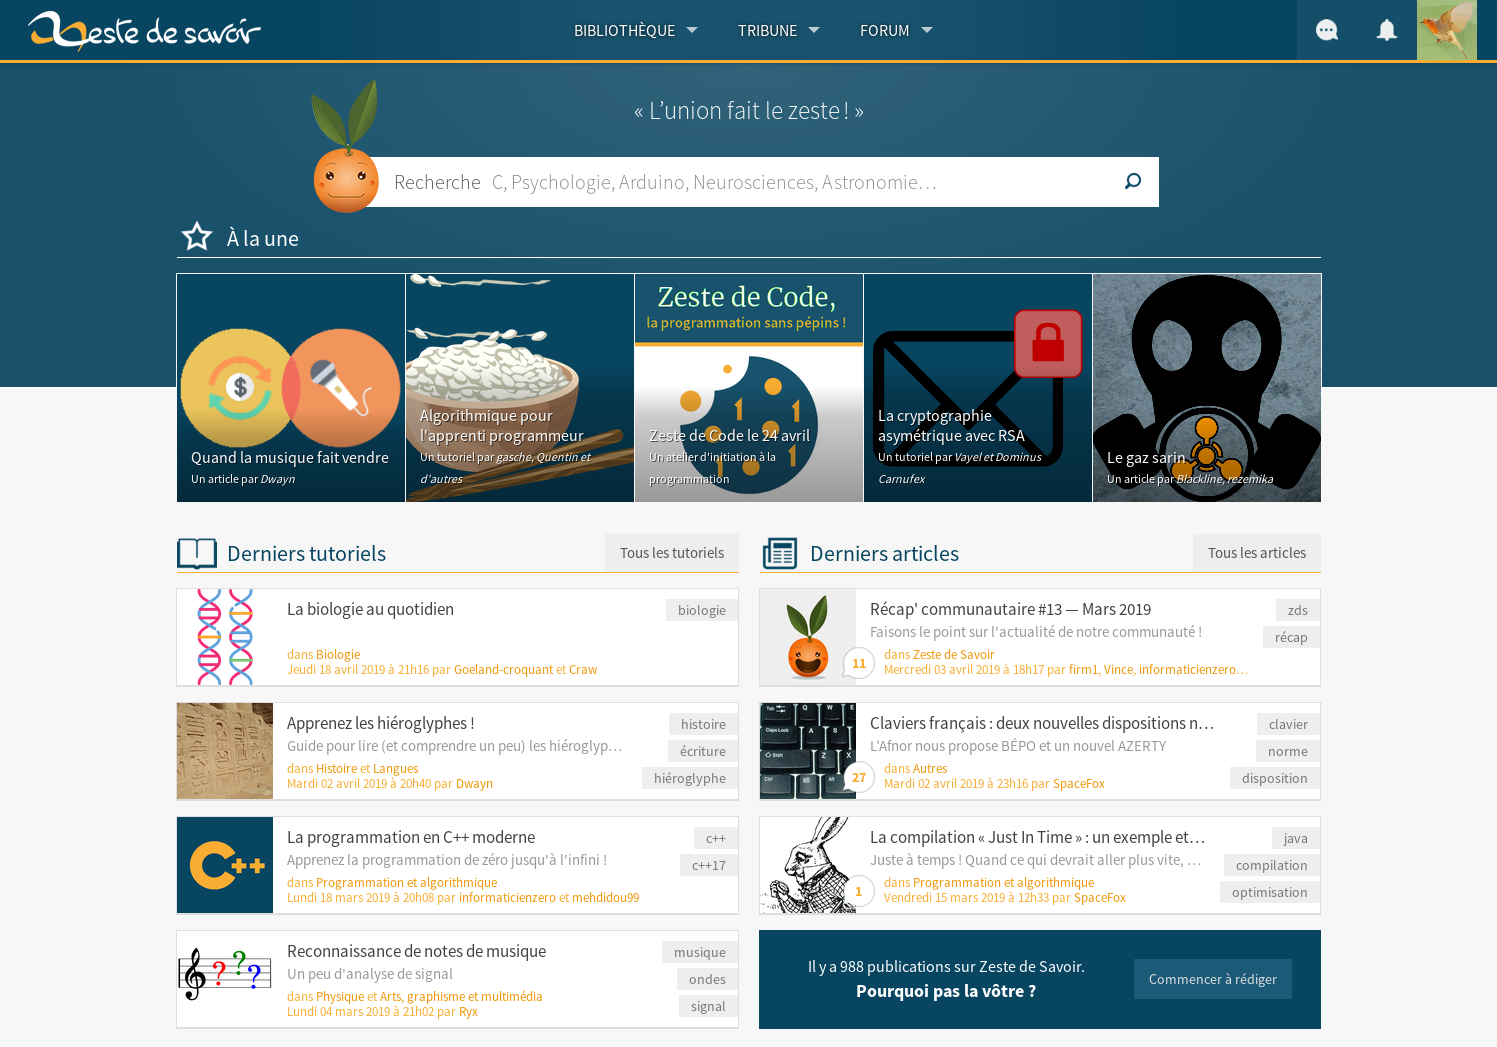
\includegraphics[width=8cm]{zeste-de-savoir-capture.png}\\
        Promouvoir le \textbf{partage de connaissances} et aider à l’auto-formation dans divers domaines, notamment informatiques et scientifiques
    \end{center}
\end{frame}

\setbeamercovered{transparent}

\begin{frame}
    \frametitle{Zeste de Savoir : qu'y trouve-t-on ?}
    \begin{itemize}
        \item<1,6> \textbf{Sciences} : physique, mathématiques, astronomie…
        \item<2,6> \textbf{Musique} : théorie musicale, débuter avec le jazz, la physique des cordes de guitare…
        \item<3,6> \textbf{Électronique} : Arduino, premiers pas dans l'informatique embarquée…
        \item<4,6> \textbf{Informatique} : apprendre à programmer avec Python (et d'autres)…
        \item<5,6> \textbf{Sciences humaines} : droit, économie, système électoral, langues…
    \end{itemize}
\end{frame}

\setbeamercovered{invisible}

\section{Atelier}

\begin{frame}
    \frametitle{Que veut dire programmer ?}

    % suboptimal but it works
    \begin{description} \item[\textbf{Programmer} (coder)] \end{description}
    
    \begin{itemize}
        \item Écrire un programme informatique
        \item Établir à l'avance une suite d'opérations ; planifier
    \end{itemize}
    
    \pause                                        
            
    \begin{description} \item[\textbf{Programme} (code)] \end{description}
    
    \begin{itemize}
     \item Description de la suite d'opérations que doit effectuer une machine
    \end{itemize}   
\end{frame}

\begin{frame}
    \frametitle{Que veut dire programmer ?}
    Concrètement, parler à l'ordinateur pour \textbf{lui dire quoi faire}
    
    \pause

    Un peu comme une \textbf{recette de cuisine} :
    \begin{itemize}
        \item casse 4 oeufs dans un saladier ;
        \item ajoute 150g de farine, 150g de sucre et 150g de beurre ;
        \item ajoute une pincée de sel et un paquet de levure ;
        \item mélange avec un fouet pendant 2 minutes ;
        \item enfourne thermostat 7 pendant 10 minutes.
    \end{itemize}
\end{frame}

\begin{frame}
    \frametitle{Quelle langue pour parler à l'ordinateur ?}
    \begin{itemize}
        \item Langues que l'humain parle : français, anglais... \pause
        \item Langue que l'ordinateur parle : binaire (001010101101)
    \end{itemize}
    
    \pause

    La solution : faire \textbf{une langue intermédiaire}
    \begin{itemize}
        \item Python
        \item Scratch
    \end{itemize}

    \begin{scriptsize}\textit{(En fait, il y en a beaucoup d'autres !)}\end{scriptsize}
\end{frame}

\begin{frame}
    \frametitle{Pourquoi programmer ?}
    \begin{itemize}
        \item Mieux comprendre le fonctionnement des ordinateurs \pause
        \item Créer des programmes (qui font ce qu'\textit{on} veut) \pause
        \item S'amuser !
    \end{itemize}
\end{frame}

\end{document}
